% A graph break for boolean subsetting: the second program's shape depends on
% a value the first program computes, so every new value is a new compile.
\documentclass[tikz, border=10pt]{standalone}
\usetikzlibrary{arrows.meta, positioning}

\begin{document}
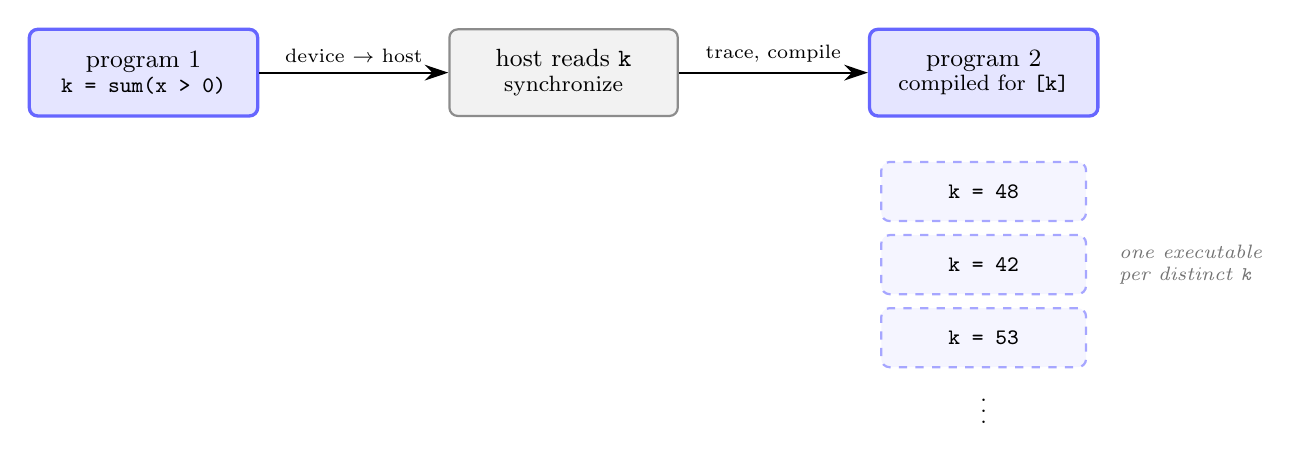
\begin{tikzpicture}[
  node distance=2.4cm,
  box/.style={
    draw, rounded corners=3pt, thick,
    minimum width=2.9cm, minimum height=1.1cm,
    align=center, font=\small
  },
  prog/.style={box, fill=blue!10, draw=blue!60, very thick},
  host/.style={box, fill=black!5, draw=black!45},
  variant/.style={box, fill=blue!4, draw=blue!35, dashed, minimum width=2.6cm, minimum height=0.75cm, font=\footnotesize},
  arr/.style={-{Stealth[length=3mm, width=2mm]}, thick},
  lab/.style={font=\scriptsize}
]
  \node[prog] (p1) {program 1\\[-2pt]{\footnotesize\texttt{k = sum(x > 0)}}};
  \node[host, right=of p1] (h) {host reads \texttt{k}\\[-2pt]{\footnotesize synchronize}};
  \node[prog, right=of h] (p2) {program 2\\[-2pt]{\footnotesize compiled for \texttt{[k]}}};

  \draw[arr] (p1) -- node[above, lab] {device $\to$ host} (h);
  \draw[arr] (h) -- node[above, lab] {trace, compile} (p2);

  \node[variant, below=0.55cm of p2] (v1) {\texttt{k = 48}};
  \node[variant, below=0.15cm of v1] (v2) {\texttt{k = 42}};
  \node[variant, below=0.15cm of v2] (v3) {\texttt{k = 53}};
  \node[font=\footnotesize, below=0.05cm of v3] {$\vdots$};
  \node[font=\scriptsize\itshape, text=black!55, align=left, anchor=west]
    at ([xshift=8pt]v2.east) {one executable\\per distinct \texttt{k}};
\end{tikzpicture}
\end{document}
